% This file was created with tikzplotlib v0.10.1.
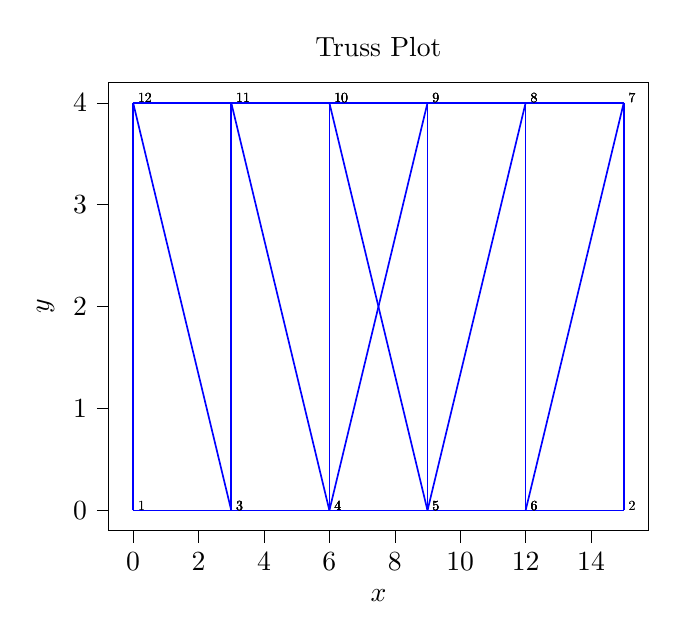
\begin{tikzpicture}

\definecolor{darkgray176}{RGB}{176,176,176}

\begin{axis}[
tick align=outside,
tick pos=left,
title={Truss Plot},
x grid style={darkgray176},
xlabel={\(\displaystyle x\)},
xmin=-0.75, xmax=15.75,
xtick style={color=black},
y grid style={darkgray176},
ylabel={\(\displaystyle y\)},
ymin=-0.2, ymax=4.2,
ytick style={color=black}
]
\addplot [semithick, blue]
table {%
0 0
0 4
};
\addplot [semithick, blue]
table {%
0 0
3 0
};
\addplot [semithick, blue]
table {%
3 0
0 4
};
\addplot [semithick, blue]
table {%
3 4
0 4
};
\addplot [semithick, blue]
table {%
3 0
3 4
};
\addplot [semithick, blue]
table {%
3 0
6 0
};
\addplot [semithick, blue]
table {%
6 0
3 4
};
\addplot [semithick, blue]
table {%
6 4
3 4
};
\addplot [semithick, blue]
table {%
6 0
6 4
};
\addplot [semithick, blue]
table {%
6 0
9 0
};
\addplot [semithick, blue]
table {%
9 0
6 4
};
\addplot [semithick, blue]
table {%
6 4
9 4
};
\addplot [semithick, blue]
table {%
9 4
9 0
};
\addplot [semithick, blue]
table {%
6 0
9 4
};
\addplot [semithick, blue]
table {%
9 0
12 0
};
\addplot [semithick, blue]
table {%
9 0
12 4
};
\addplot [semithick, blue]
table {%
12 0
12 4
};
\addplot [semithick, blue]
table {%
12 4
9 4
};
\addplot [semithick, blue]
table {%
12 4
15 4
};
\addplot [semithick, blue]
table {%
12 0
15 4
};
\addplot [semithick, blue]
table {%
15 0
15 4
};
\addplot [semithick, blue]
table {%
15 0
12 0
};
\draw (axis cs:0,0) node[
  scale=0.5,
  anchor=base west,
  text=black,
  rotate=0.0
]{1};
\draw (axis cs:0,4) node[
  scale=0.5,
  anchor=base west,
  text=black,
  rotate=0.0
]{12};
\draw (axis cs:0,0) node[
  scale=0.5,
  anchor=base west,
  text=black,
  rotate=0.0
]{1};
\draw (axis cs:3,0) node[
  scale=0.5,
  anchor=base west,
  text=black,
  rotate=0.0
]{3};
\draw (axis cs:3,0) node[
  scale=0.5,
  anchor=base west,
  text=black,
  rotate=0.0
]{3};
\draw (axis cs:0,4) node[
  scale=0.5,
  anchor=base west,
  text=black,
  rotate=0.0
]{12};
\draw (axis cs:3,4) node[
  scale=0.5,
  anchor=base west,
  text=black,
  rotate=0.0
]{11};
\draw (axis cs:0,4) node[
  scale=0.5,
  anchor=base west,
  text=black,
  rotate=0.0
]{12};
\draw (axis cs:3,0) node[
  scale=0.5,
  anchor=base west,
  text=black,
  rotate=0.0
]{3};
\draw (axis cs:3,4) node[
  scale=0.5,
  anchor=base west,
  text=black,
  rotate=0.0
]{11};
\draw (axis cs:3,0) node[
  scale=0.5,
  anchor=base west,
  text=black,
  rotate=0.0
]{3};
\draw (axis cs:6,0) node[
  scale=0.5,
  anchor=base west,
  text=black,
  rotate=0.0
]{4};
\draw (axis cs:6,0) node[
  scale=0.5,
  anchor=base west,
  text=black,
  rotate=0.0
]{4};
\draw (axis cs:3,4) node[
  scale=0.5,
  anchor=base west,
  text=black,
  rotate=0.0
]{11};
\draw (axis cs:6,4) node[
  scale=0.5,
  anchor=base west,
  text=black,
  rotate=0.0
]{10};
\draw (axis cs:3,4) node[
  scale=0.5,
  anchor=base west,
  text=black,
  rotate=0.0
]{11};
\draw (axis cs:6,0) node[
  scale=0.5,
  anchor=base west,
  text=black,
  rotate=0.0
]{4};
\draw (axis cs:6,4) node[
  scale=0.5,
  anchor=base west,
  text=black,
  rotate=0.0
]{10};
\draw (axis cs:6,0) node[
  scale=0.5,
  anchor=base west,
  text=black,
  rotate=0.0
]{4};
\draw (axis cs:9,0) node[
  scale=0.5,
  anchor=base west,
  text=black,
  rotate=0.0
]{5};
\draw (axis cs:9,0) node[
  scale=0.5,
  anchor=base west,
  text=black,
  rotate=0.0
]{5};
\draw (axis cs:6,4) node[
  scale=0.5,
  anchor=base west,
  text=black,
  rotate=0.0
]{10};
\draw (axis cs:6,4) node[
  scale=0.5,
  anchor=base west,
  text=black,
  rotate=0.0
]{10};
\draw (axis cs:9,4) node[
  scale=0.5,
  anchor=base west,
  text=black,
  rotate=0.0
]{9};
\draw (axis cs:9,4) node[
  scale=0.5,
  anchor=base west,
  text=black,
  rotate=0.0
]{9};
\draw (axis cs:9,0) node[
  scale=0.5,
  anchor=base west,
  text=black,
  rotate=0.0
]{5};
\draw (axis cs:6,0) node[
  scale=0.5,
  anchor=base west,
  text=black,
  rotate=0.0
]{4};
\draw (axis cs:9,4) node[
  scale=0.5,
  anchor=base west,
  text=black,
  rotate=0.0
]{9};
\draw (axis cs:9,0) node[
  scale=0.5,
  anchor=base west,
  text=black,
  rotate=0.0
]{5};
\draw (axis cs:12,0) node[
  scale=0.5,
  anchor=base west,
  text=black,
  rotate=0.0
]{6};
\draw (axis cs:9,0) node[
  scale=0.5,
  anchor=base west,
  text=black,
  rotate=0.0
]{5};
\draw (axis cs:12,4) node[
  scale=0.5,
  anchor=base west,
  text=black,
  rotate=0.0
]{8};
\draw (axis cs:12,0) node[
  scale=0.5,
  anchor=base west,
  text=black,
  rotate=0.0
]{6};
\draw (axis cs:12,4) node[
  scale=0.5,
  anchor=base west,
  text=black,
  rotate=0.0
]{8};
\draw (axis cs:12,4) node[
  scale=0.5,
  anchor=base west,
  text=black,
  rotate=0.0
]{8};
\draw (axis cs:9,4) node[
  scale=0.5,
  anchor=base west,
  text=black,
  rotate=0.0
]{9};
\draw (axis cs:12,4) node[
  scale=0.5,
  anchor=base west,
  text=black,
  rotate=0.0
]{8};
\draw (axis cs:15,4) node[
  scale=0.5,
  anchor=base west,
  text=black,
  rotate=0.0
]{7};
\draw (axis cs:12,0) node[
  scale=0.5,
  anchor=base west,
  text=black,
  rotate=0.0
]{6};
\draw (axis cs:15,4) node[
  scale=0.5,
  anchor=base west,
  text=black,
  rotate=0.0
]{7};
\draw (axis cs:15,0) node[
  scale=0.5,
  anchor=base west,
  text=black,
  rotate=0.0
]{2};
\draw (axis cs:15,4) node[
  scale=0.5,
  anchor=base west,
  text=black,
  rotate=0.0
]{7};
\draw (axis cs:15,0) node[
  scale=0.5,
  anchor=base west,
  text=black,
  rotate=0.0
]{2};
\draw (axis cs:12,0) node[
  scale=0.5,
  anchor=base west,
  text=black,
  rotate=0.0
]{6};
\end{axis}

\end{tikzpicture}
